\chapter{Methodology}
\label{Chapter5}
\lhead{Chapter 5. \emph{Methodology}}

\section{Overview}

To address the architectural flaws identified in the initial framework (Chapter~4), \textbf{the enhanced AgentClinic framework} was developed as a complete redesign of the multi-agent clinical simulation system. This chapter presents the formal POMDP model, the functional agent definitions, the LangGraph finite-state orchestration, the hardware adaptation strategy, and the formulation of process-oriented evaluation metrics.




\section{Formalizing the Clinical Agent System}

The interactive diagnostic process naturally maps to a Partially Observable Markov Decision Process (POMDP). At each timestep $t$, the true patient state $s_t$ (the underlying disease) is hidden from the Doctor agent. The Doctor must instead infer the diagnosis through a sequence of observations and actions. The AgentClinic system is formally defined as a tuple $M = \langle S, A, T, R, \Omega, O \rangle$:
\begin{itemize}
    \item \textbf{State Space ($S$):} The clinical ground truth, encompassing the patient's actual disease, symptoms, and physiological parameters.
    \item \textbf{Action Space ($A$):} The actions available to the Doctor agent, including asking a question ($a_{\text{dialogue}}$), ordering a test ($a_{\text{test}}$), or rendering a final diagnostic verdict ($a_{\text{diagnosis}}$).
    \item \textbf{Transition Function ($T$):} The progression of the conversation and the internal physiological timeline of the patient over $t$.
    \item \textbf{Reward Function ($R$):} The framework does not currently incorporate active reinforcement learning optimization during dialogue. Instead, $R$ is computed retrospectively via the \texttt{ClinicalTrajectoryEvaluator} strictly for offline evaluation, penalizing inefficiency (IE), erratic hypotheses (DS), and unsafe test orders (TR).
    \item \textbf{Observation Space ($\Omega$):} The text outputs produced by the Patient agent (symptom descriptions) and the Measurement agent (test results).
    \item \textbf{Observation Function ($O$):} The mapping of true states to natural language observations, perturbed by the Patient agent's persona.
\end{itemize}



\section{Defining the Functional Agents}

Execution is delegated to four highly constrained and functionally isolated agents:

\subsection{Doctor Agent}
The Doctor Agent operates the medical policy $\pi$. Its objective is to actively collapse diagnostic uncertainty. It engages in:
\begin{itemize}
    \item Sequential history-taking using conversational queries.
    \item Metacognitive reflection, emitting top-three structured hypotheses before speaking.
    \item Evidence acquisition via targeted clinical test orders.
    \item Synthesis of a final diagnostic verdict within a strictly bounded interaction threshold ($N_{\text{max\_infs}} = 10$).
\end{itemize}

\subsection{Patient Agent}
The Patient Agent functions as the observation emission generator $O(s_t, a_t)$. Parameterised by the hidden OSCE scenario state, it:
\begin{itemize}
    \item Provides accurate physiological data bounded exclusively to the assigned case scenario.
    \item Generates responses explicitly restricted to short 1--3 sentence conversational bounds.
    \item Absorbs patient-side bias injections (e.g., anxiety, guardedness) which mathematically distort the observation function.
\end{itemize}

\subsection{Measurement Agent}
The Measurement Agent acts as a deterministic oracle returning physiological ground truth. It:
\begin{itemize}
    \item Parses test requests using combined rule-based logic and semantic text matching.
    \item Returns structured laboratory results, numerical vitals, and examination strings if the requested test correlates with the clinical condition.
    \item Emits ``NORMAL READINGS'' if a structurally valid test yields no pathology, forcing the Doctor to correctly interpret negative findings.
\end{itemize}

\subsection{Moderator Agent}
The Moderator Agent functions as an objective semantic judge utilized exclusively at the terminal state $t_{\text{end}}$. It:
\begin{itemize}
    \item Takes the Doctor's final output and the hidden ground-truth diagnosis as inputs.
    \item Computes semantic equivalence, accommodating synonymy and partial phrasing without penalizing clinically valid linguistic variation.
    \item Outputs a strict binary (Yes/No) correctness flag, calculating the episode reward for the $R$ function.
\end{itemize}

\section{Implementation via Finite-State Orchestration}

The core limitation of the prior ad-hoc loop was its inability to enforce strict, deterministic state transitions. In the enhanced framework, LangGraph was adopted strictly as the \textit{execution substrate} to enforce the theoretical POMDP state machine. The consultation protocol executes as a Directed Cyclic Graph (DCG) finite-state controller. Nodes represent the functional agents, and edges encode deterministic routing logic conditioned on the active phase of consultation.

\subsection{State Initialisation and Reducers}

\paragraph{Definition of ClinicalState:}
The \texttt{ClinicalState} dictionary tracks the sequential progression of the POMDP execution and bounds the dynamic context window. It consists of the following core fields:
\begin{itemize}
    \item \texttt{last\_input\_to\_doctor}: The most recent response from the patient or measurement agent.
    \item \texttt{last\_doctor\_message}: The doctor's most recent interaction.
    \item \texttt{differential\_diagnoses}: The latent JSON array of the top-three diagnoses.
    \item \texttt{turn\_count}: A counter enforcing the $\max_{\text{infs}}$ threshold.
    \item \texttt{diagnosis\_ready}: A flag indicating terminal closure.
    \item \texttt{differential\_trajectory}: Accumulated hypothesis snapshots for metric evaluation.
    \item \texttt{tests\_ordered}: Registry of formally requested diagnostics.
    \item \texttt{full\_dialogue}: The complete chronologically ordered text transcript.
\end{itemize}
State transitions are strictly governed by non-destructive \textit{reducers} to ensure observations are updated without overwriting prior evidence.

Execution of the graph relies on this formally defined vector, handled deterministically by the LangGraph orchestrator.

\subsection{The Latent Metacognitive Reflection Node}

The most important architectural change is the introduction of the \texttt{doctor\_reflection} node. Human clinicians maintain a mental differential diagnosis that evolves silently as they interview a patient. Standard LLMs have no equivalent scratchpad; when forced to generate bedside dialogue and medical reasoning simultaneously, they tend to hallucinate or leak internal reasoning into spoken dialogue.

\paragraph{Decoupling Reasoning from Generation (Latent Chain-of-Thought):}
Standard auto-regressive LLMs compute the probability of each token conditioned on all preceding tokens: $P(w_t \mid w_1, \ldots, w_{t-1})$. When a model is asked to simultaneously generate bedside dialogue and perform complex multi-conditional reasoning, its self-attention heads must split capacity between syntactic fluency and semantic medical deduction. 

In the enhanced framework, the \texttt{doctor\_reflection} node acts as a \textit{Latent Chain-of-Thought (CoT) mechanism}~\cite{wang2024survey}. The DCG routes execution to the \texttt{doctor\_reflection} node before any spoken utterance. Here, the LLM outputs a structured JSON array of its current top-3 differential diagnoses (e.g., \texttt{["Asthma", "COPD", "Pneumonia"]}), operating at a low sampling temperature ($T=0.1$) to ensure deterministic extraction. These hypotheses are stored in the \texttt{ClinicalState} trajectory log but are \textit{not} injected into the patient-facing dialogue history. High-information medical tokens are injected directly into the context window. When the \texttt{doctor\_speaker} node subsequently executes, its attention heads attend heavily to this structured JSON, constraining the dialogue distribution to align with the prior diagnostic reasoning without contaminating the interaction.

\begin{figure}[htbp]
\centering
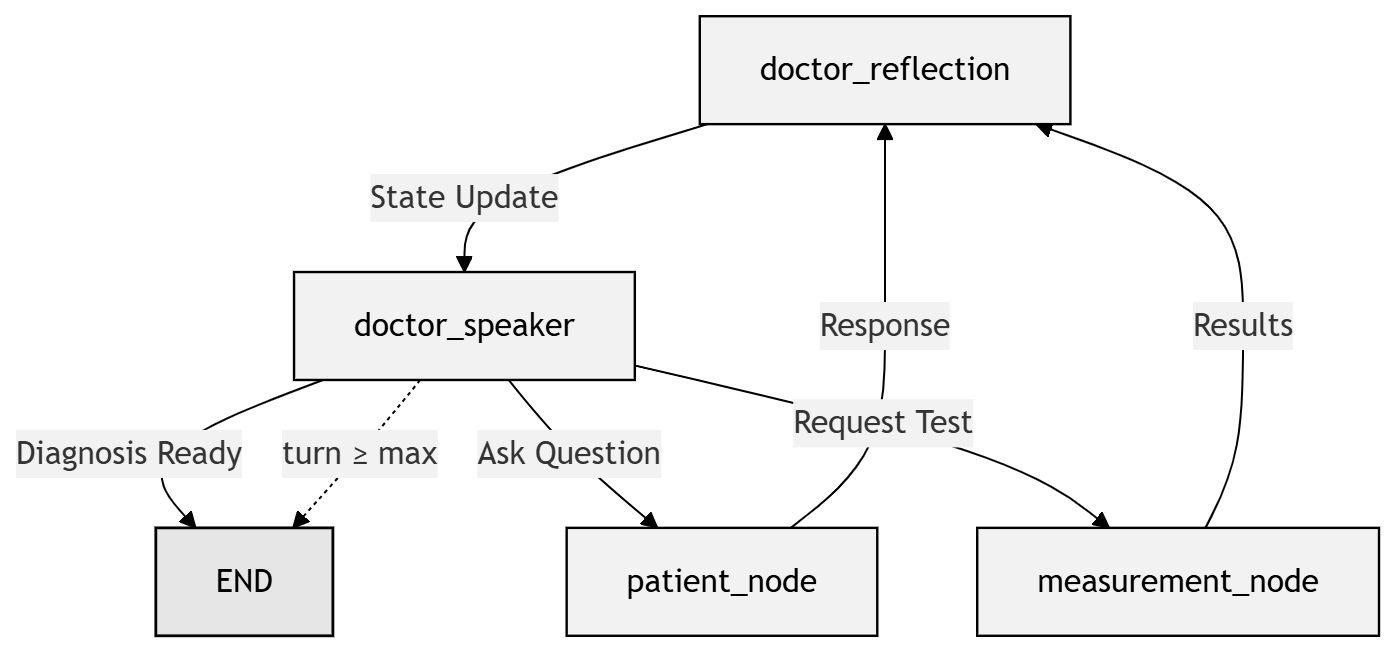
\includegraphics[width=\textwidth]{Pictures/LangGraph.png}
\caption{LangGraph DCG topology of the enhanced framework. The \texttt{doctor\_reflection} node ensures reasoning trajectories are recorded systematically before each spoken turn, providing a structured metacognitive mechanism without contaminating patient-facing dialogue.}
\label{fig:langgraph}
\end{figure}

\subsection{Doctor Speaker Node}
Following the reflection phase, the finite-state machine transitions to the \texttt{doctor\_speaker} node. This node inherits the \texttt{ClinicalState}, including the newly generated latent diagnostic JSON array. The Doctor agent is then prompted to emit a single conversational utterance directed at the patient. Because the prior reasoning is already present in the context, the model's self-attention layers naturally condition the spoken generation on the latent hypotheses, yielding targeted, clinically sound history-taking without overt hallucination.

\subsection{Patient Statement Node}
The \texttt{patient\_node} acts primarily as an observation generator. It is invoked when the Doctor emits a conversational question. The node passes the accumulated dialogue history to the Patient LLM, which is rigidly bounded by the background case scenario. It generates a 1--3 sentence symptom report or response (the observation), which the LangGraph orchestrator subsequently appends to the conversation history before looping back to the Doctor.

\subsection{Measurement Execution Node}
When the Doctor outputs a structural \texttt{REQUEST TEST} command rather than conversational dialogue, the orchestrator routes execution to the \texttt{measurement\_node}. Operating deterministically, this node intercepts the test string, performs rule-based and semantic validation against the hidden case record, and returns the corresponding clinical findings. The result is appended to the context window as objective physiological data for the Doctor's subsequent reflection step.

\section{Hardware Adaptation}

To eliminate \textit{Lexical Leakage}, the enhanced framework follows a \textit{Cognitive Asymmetry} design principle: the Doctor operates as a domain-expert engine, while the Patient, Measurement, and Moderator agents run on separate, architecturally distinct model instances.

Running three or more distinct 7B-parameter models simultaneously on a single NVIDIA H100 NVL (95.8\,GB VRAM) imposes strict hardware constraints. To deploy the theoretical multi-agent model onto consumer or single-node hardware without exceeding VRAM bounds, the weight matrices were adapted using \textbf{NormalFloat4 (NF4) quantisation} via the BitsAndBytes library~\cite{dettmers2023qlora}. While not a novel algorithmic contribution of this thesis, applying NF4 transforms neural network weights---which naturally approximate a zero-mean normal distribution---into an information-theoretically optimal 4-bit projection for inference.

This hardware adaptation reduces the memory footprint per 7B model by approximately 86.4\%, rendering heterogeneous multi-engine isolation operational and leaving sufficient buffer for Flash Attention 2 context scaling.

\section{Robust LLM Output Extraction and Fallbacks}

To ensure the LangGraph state machine operates deterministically even when the LLMs produce structurally malformed strings, programmatic guardrails were implemented to address the fragility of raw text generation.

\subsection{Multi-level JSON Extraction}
A cascading heuristic extraction utility prevents pipeline termination when the \texttt{doctor\_reflection} node hallucinates escaping characters. It cascades through a programmatic fallback:
\begin{enumerate}
    \item Strict JSON parsing.
    \item Regular expression bracket matching to isolate arrays.
    \item Comma-splitting heuristics for unquoted sequences.
    \item Quoted string heuristic extraction.
\end{enumerate}

\subsection{Forced Diagnostic Closure Fallback}
If the Doctor agent exhausts its token context window or fails to emit a \texttt{DIAGNOSIS\_READY} flag after the maximum allowed turns ($N_{\text{max\_infs}} = 10$), the graph prevents a silent failure by routing to a forced programmatic closure trigger. This injects an aggressive few-shot prompt forcing immediate diagnostic closure based on the accumulated \texttt{ClinicalState}.

\subsection{Cross-Model Prompt Alignment}
Given the deployment of heterogeneous models (e.g., Mistral vs. Llama architectures), hardcoded prompt formatting causes catastrophic degradation due to mismatched instruction tokens. The HuggingFace \texttt{apply\_chat\_template()} utility was utilized to dynamically map generic dialogue arrays into the precise control token formats required by each specific engine constraint.

\section{Formulation of Process-Oriented Clinical Metrics}

Binary diagnostic accuracy alone can mask serious reasoning flaws. The \texttt{ClinicalTrajectoryEvaluator} computes three process-oriented metrics inline, using data accumulated in the \texttt{ClinicalState} trajectory.

\paragraph{1. Diagnostic Stability (DS):} Measures the mean Jaccard similarity between consecutive differential diagnoses over $T$ turns. High stability suggests logical hypothesis refinement; low stability signals erratic switching. Its use is justified to mathematically quantify a model's resistance to recency bias and arbitrary hypothesis switching during prolonged interactions.
\begin{equation}
\text{DS} = \frac{1}{T - 1} \sum_{t=1}^{T-1} \frac{|\text{DDx}_t \cap \text{DDx}_{t+1}|}{|\text{DDx}_t \cup \text{DDx}_{t+1}|}
\end{equation}


\paragraph{2. Test Rationality (TR):} A binary compliance indicator that checks whether the model ordered at least one basic investigation (e.g., CBC, vitals) before requesting expensive or invasive procedures (e.g., MRI, biopsy). Its justification stems from the clinical mandate to follow stepwise diagnostic guidelines, penalizing LLMs that exhibit premature diagnostic closure or unsafe invasive test generation. Let $t_{\text{basic}}$ and $t_{\text{adv}}$ represent basic and advanced tests, respectively:
\begin{equation}
\text{TR} = \begin{cases}
0 & \text{if } \exists\, t_{\text{adv}} \text{ ordered before any } t_{\text{basic}} \\
1 & \text{otherwise}
\end{cases}
\end{equation}


\paragraph{3. Information Efficiency (IE):} The ratio of unique differential hypotheses generated ($N_{\text{unique}}$) to the total dialogue turns utilised ($T$). Higher IE indicates greater hypothesis diversity per turn. This metric is utilised to evaluate the generative capacity of the latent reasoning node, ensuring the model effectively explores the hypothesis space without stalling:
\begin{equation}
\text{IE} = \frac{N_{\text{unique}}}{T}
\end{equation}


\section{Cognitive Bias Injections}

The enhanced framework carries forward and enhances the bias injections from the initial framework. Instead of generic sentence-level prompts, ecologically valid distortions are injected:

\begin{itemize}
    \item \textbf{Recency Bias:} The system maintains a running queue of the $k=5$ most recently processed case summaries. These are injected into the Doctor's system prompt, mimicking a physician overly influenced by recent clinical encounters. This exploits the transformer's natural tendency to assign elevated attention weights to tokens near the current generation boundary.
    \item \textbf{Confirmation Bias:} The Doctor is primed with a strong, incorrect initial hypothesis (e.g., \textit{``You are initially confident the patient has malignancy.''}). This warps the model's forward probability distribution toward confirmatory evidence acquisition, operationalising the premature diagnostic closure seen in anchoring studies.
\end{itemize}

\section{Synthetic Data Generation and LoRA Adapter Training}

To address the catastrophic forgetting observed in narrowly fine-tuned models, a parameter-efficient architecture was engineered utilizing the dynamic routing of task-specific Low-Rank Adaptation (LoRA) adapters. A major challenge in fine-tuning clinical inference engines is the scarcity of high-quality, annotated differential diagnosis trajectories and empathetic clinical dialogues.

\subsection{Synthetic Data Generation (SDG) Pipeline}
To resolve this data scarcity, a deterministic Synthetic Data Generation (SDG) pipeline was built utilizing the base OSCE scenarios from the NEJM case subset. The pipeline programmatically extracts case vignettes and utilizes a high-capacity teacher model to synthesize distinct training corpora:
\begin{enumerate}
    \item \textbf{Reasoning Corpus:} Generated via a deterministic prompt engineering procedure that synthesizes structured JSON arrays of top-three differential diagnoses grounded in the vignette's physiological state.
    \item \textbf{Dialogue Corpus:} Generated via a conditional dialogue synthesis procedure that produces multi-turn empathetic conversational transcripts demonstrating targeted history-taking.
\end{enumerate}

\subsection{QLoRA SFTTrainer Configuration}
Two lightweight adapters were trained independently utilizing the HuggingFace \texttt{SFTTrainer} and \texttt{PEFT} libraries~\cite{wolf2020huggingfaces}. The base model was loaded in 4-bit NF4 precision while the adapters were trained in \texttt{bf16}. LoRA adapters ($r=16$, $\alpha=32$) were applied to all four attention projection matrices (\texttt{q\_proj}, \texttt{k\_proj}, \texttt{v\_proj}, \texttt{o\_proj}) across all transformer layers. The training utilized the AdamW optimizer with a learning rate of $2 \times 10^{-4}$ and 4-step gradient accumulation.

\begin{itemize}
    \item The \textit{reasoning adapter} is activated exclusively during the \texttt{doctor\_reflection} node to steer the latent probability distribution toward structured diagnostic enumeration.
    \item The \textit{dialogue adapter} is activated during the \texttt{doctor\_speaker} node to retrieve conversational fluency.
\end{itemize}

\textbf{Data Separation for Experimental Validity:} To prevent train-test contamination, the adapters were trained strictly on NEJM scenarios, while empirical evaluations (such as the architectural extension E6) utilized the independent 107 MedQA scenarios exclusively. At inference time, the DCG dynamically swaps the active weights prior to execution of each respective node. The adapter swap is a pointer operation that redirects which $BA$ matrices are added to the frozen $W_0$. The combined VRAM overhead of both adapters is approximately 50\,MB.

